\documentclass[10pt,a4paper,headsepline,smallheadings]{scrartcl}
\usepackage[utf8]{inputenc}
\usepackage[T1]{fontenc}
\usepackage[ngerman]{babel}
\usepackage{amsmath}
\usepackage{amsthm}
\usepackage{amssymb}
\usepackage{amsfonts}
\usepackage[scaled]{helvet}
\usepackage{amssymb}
\usepackage{multirow}
\usepackage{textcomp}
\usepackage{graphicx}
\usepackage{paralist}
\usepackage{textcomp}
\usepackage{pdflscape} 
\usepackage{marvosym}
\usepackage{float}
\usepackage{siunitx}
\usepackage[siunitx,european,cuteinductors,smartlabels]{circuitikz}
\usepackage{fancyhdr}
\usepackage{pgfplots}
\usepackage{sansmath}
\usepackage{lscape}
\usepackage{multicol}

\usetikzlibrary{calc}


\theoremstyle{definition}
\newtheorem{aufgabe}{Aufgabe}


\renewcommand*\familydefault{\sfdefault}
\renewcommand{\arraystretch}{1.1}


\KOMAoptions{parskip=half,DIV=15,fontsize=11pt}
\unitlength1cm
\titlehead{

\begin{center}\begin{tabular}{p{10cm}p{6.8cm}}
\textbf{FH Aachen} & \textbf{FB Maschinenbau und Mechatronik}\\[0.5cm]
\textbf{Modul 86512} &  Prof. Dr. Raphael Pfaff\\
Herstellung und Vermarktung& Sommersemester 2015\\
\end{tabular}

\end{center}
\begin{picture}(0,0)(0,0)\put(17,-23){
\includegraphics[height=5cm]{fh_logo}}\end{picture}
}
\newif\ifuelsg %als slides
%\uelsgtrue
\uelsgfalse
\newif\ifnotuelsg
\ifuelsg\notuelsgfalse\else\notuelsgtrue\fi
\graphicspath{
{../Bilder/Uebungen/}
{../Bilder/Wirkungsplan/}
}

%\titlehead{83105 \hfill Mess-Steuerungs- und Regelungstechnik \hfill Prof. Manfred Enning}
\title{Herstellung und Vermarktung von Schienenfahrzeugen  -- \"Ubung 3}
\date{}
\makeatletter
\let\Title\@title
\let\Author\@author
\makeatother
\pagestyle{fancy}
\fancyhead[LE, LO]{Prof. Dr. Raphael Pfaff}
\fancyhead[RE, RO]{\Title}

\begin{document}
\thispagestyle{empty}
\maketitle
\vspace{-2cm}
% \hyphenation{Abwei-chungen}

\section*{Schraubenberechnung}

\begin{center}
            		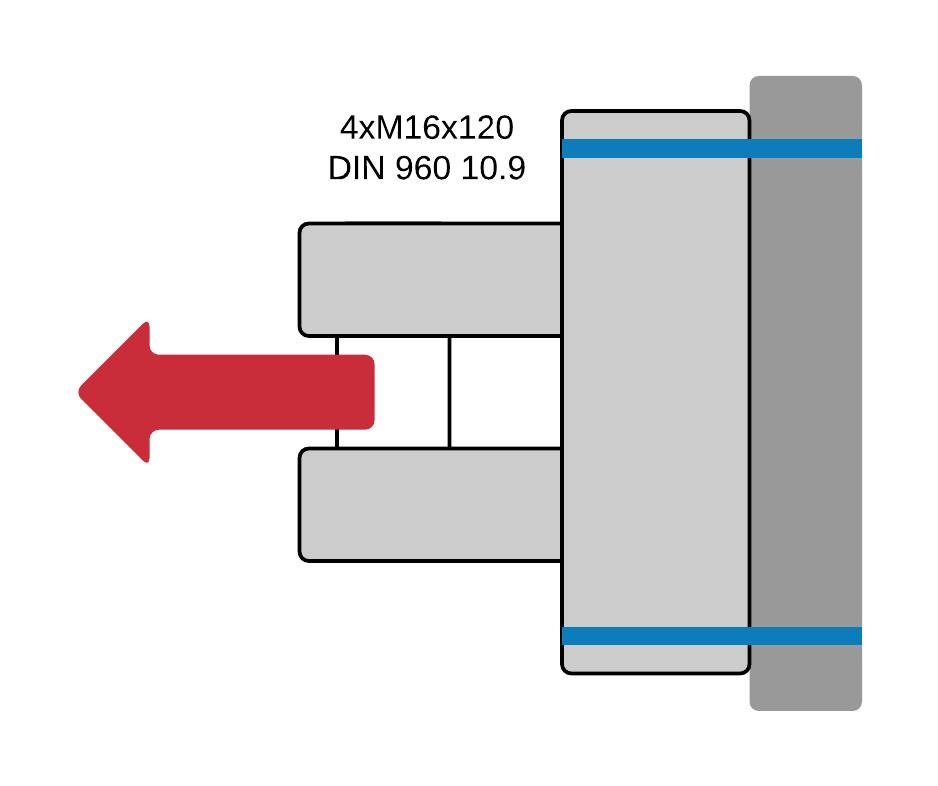
\includegraphics[width=0.38\textwidth]{KonsoleKupplung}
		
        		\end{center}

\begin{aufgabe}[Analytische Schraubenberechnung. Gruppenarbeit 2-3] 

         	
   
Die Schraubenverbindung (Feingewinde) wie im Bild dargestellt wurde mittels ausl\"osendem Drehmomentschl\"ussel nach Sch\"atzung der Reibungsverh\"altnisse montiert. Dabei wurde die maximale Schraubenvorspannung so gew\"ahlt, dass 90 \% der Mindeststreckgenze ausgenutzt werden.

Die verschraubten Teile bestehen aus Stahl, die Montage erfolgt gereinigt. Es sind keine statischen und Setzeffekte zu ber\"ucksichtigen.

Im Feld kommt es zu Querverschiebungen der Konsole und Versagen der Schraubenverbindung durch Querbelastung. Der maximale Auslenkwinkel betr\"agt $\gamma = 15^{\circ}$. 

\begin{enumerate}[a)]
\item Ermitteln Sie eine potenzielle Root-Cause mittels eines Ishikawa-Diagramms mit den Kategorien:
	\begin{itemize}
		\item Mensch
		\item Maschine
		\item Methode
		\item Management
		\item Mitwelt
	\end{itemize}
\item Ermitteln Sie eine potenzielle Root-Cause mittels 5-Why-Fragen.
\end{enumerate}
\end{aufgabe}
\newpage
\begin{aufgabe}[Analytische Schraubenberechnung. Gruppenarbeit 2-3] 
Die Aufgabe bezieht sich ebenfalls auf die oben dargestellte Verschraubung.
\begin{enumerate}[a)]
\item Geben Sie die Risikoklasse der Verschraubung an.
\item Bestimmen Sie die minimale und maximale Klemmkraft einer Schraubverbindung unter Ber\"ucksichtigung des Anziehfaktors $\alpha_{A}$.
\item Welche Zugkraft gen\"ugt, um eine Entlastung der Konsole zu bewirken, unter Annahme der ung\"unstigsten Verschraubung. 
\item Welche Zugkraft kann von der dargestellten Verbindung unter Annahme des maximalen Schwenkwinkels \"ubertragen werden ohne eine Querverschiebung zu bewirken?
\end{enumerate}

\end{aufgabe}
\end{document}